\newpage
\subsection{Wersja 1}

\subsubsection{Opis rozwiązania}

W pierwszej wersji programu wykorzystany został tylko jeden blok wątków. Każdy z wątków oblicza\footnotemark $$\frac{\text{szerokość macierzy}}{\text{szerokość bloku}} \times \frac{\text{wysokość macierzy}}{\text{wysokość bloku}}$$ elementów wyniku. Pamięć współdzielona nie jest wykorzystywana.
\footnotetext{W analizowanych przypadkach wysokość macierzy jest równa szerokości macierzy, wysokość bloku jest równa szerokości bloku.}

\lstinputlisting[caption=Mnożenie macierzy kwadratowych na GPU -- wersja 1.]{./code/matrix_multiplication_1.cpp}

\newpage
\subsubsection{Teoretyczna zajętość SM}

\begin{center}
\begin{table}[H]
\centering
\begin{tabular}{|c|c|c|c|c|c|}
\hline
\multicolumn{2}{|c|}{\multirow{2}{*}{Kryterium}} & \multicolumn{3}{c|}{Teoretyczna wartość} & \multirow{2}{*}{Limit GPU} \\ \cline{3-5}
\multicolumn{2}{|c|}{} & 8x8 & 16x16 & 22x22 & \\ \hline
\multirow{4}{*}{Zajętość SM} & Aktywne bloki & 1 & 1 & 1 & 8 \\ \cline{2-6}
& Aktywne warpy & 2 & 8 & 16 & 32 \\ \cline{2-6}
& Aktywne wątki & 64 & 256 & 484 & 1024 \\ \cline{2-6}
& Zajętość & 6.25\% & 25.00\% & 50.00\% & 100.00\% \\ \hline
\multirow{2}{*}{Warpy} & Wątki/Blok & 64 & 256 & 484 & 512 \\ \cline{2-6}
& Warpy/Blok & 2 & 8 & 16 & 16 \\ \hline
\multirow{2}{*}{Rejestry} & Rejestry/Wątek & 16 & 16 & 16 & 128 \\ \cline{2-6}
& Rejestry/Blok & 1024 & 4096 & 8192 & 16384 \\ \hline
\multirow{1}{*}{Pamięć współdzielona} & Pamięć współdzielona/Blok & 44 & 44 & 44 & 16384 \\ \hline
\end{tabular}
\caption{Teoretyczna zajętość SM -- wersja 1.}
\end{table}
\end{center}

Wykorzystywany jest 1 blok, zatem zajętość SM warpami jest zależna tylko od jego rozmiaru.

\newpage
\subsubsection{Wyniki pomiarów}

\begin{enumerate}

\item \textbf{Czas trwania obliczeń} \newline
\begin{table}[H]
\centering
\begin{tabular}{|c|c|c|c|}
\hline
\multirow{2}{*}{Rozmiar macierzy} & \multicolumn{3}{c|}{Rozmiar bloku} \\ \cline{2-4}
& 8x8 & 16x16 & 22x22 \\ \hline
176x176 & 49.860 & 13.156 & 7.454 \\ \hline
352x352 & 398.426 & 104.408 & 59.424 \\ \hline
528x528 & 1345.355 & 349.936 & 200.265 \\ \hline
\end{tabular}
\caption{Czas obliczeń [ms] -- wersja 1.}
\end{table}

\begin{figure}[H]
\centering
  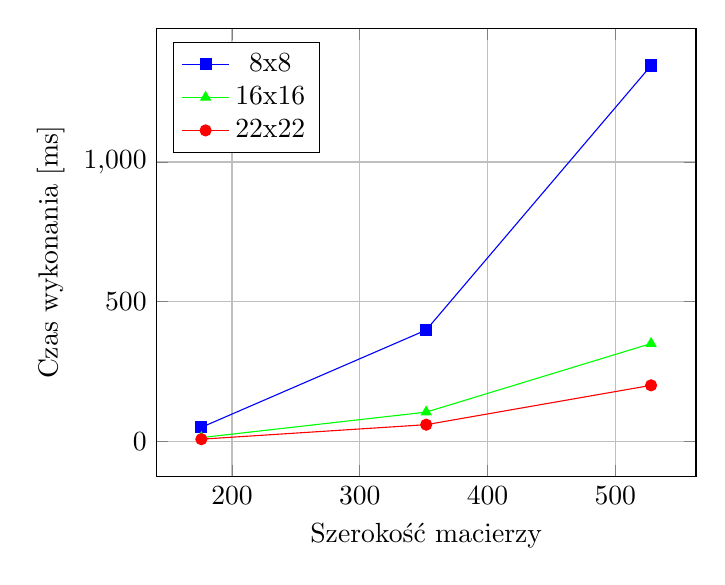
\begin{tikzpicture}
    \begin{axis}[
      xlabel=Szerokość macierzy,
      ylabel={Czas wykonania [ms]},
      legend pos=north west,
      grid=both
    ]

    \addplot[color=blue,mark=square*] coordinates {%
      (176, 49.860)
      (352, 398.426)
      (528, 1345.355)
    };
    \addlegendentry{8x8}

    \addplot[color=green,mark=triangle*] coordinates {%
      (176, 13.156)
      (352, 104.408)
      (528, 349.936)
    };
    \addlegendentry{16x16}

    \addplot[color=red,mark=*] coordinates {%
      (176, 7.454)
      (352, 59.424)
      (528, 200.265)
    };
    \addlegendentry{22x22}

    \end{axis}%
  \end{tikzpicture}%
\caption{Zależność pomiędzy ilością operacji zmiennoprzecinkowychna sekundę a rozmiarem macierzy -- wersja 3.}
\end{figure}

\newpage
\item \textbf{Ilość operacji zmiennoprzecinkowych na sekundę} \newline

\begin{table}[H]
\centering
\begin{tabular}{|c|c|c|c|}
\hline
\multirow{2}{*}{Rozmiar macierzy} & \multicolumn{3}{c|}{Rozmiar bloku} \\ \cline{2-4}
& 8x8 & 16x16 & 22x22 \\ \hline
176x176 & 0.219 & 0.829 & 1.463 \\ \hline
352x352 & 0.219 & 0.835 & 1.468 \\ \hline
528x528 & 0.219 & 0.841 & 1.470 \\ \hline
\end{tabular}
\caption{Ilość operacji zmiennoprzecinkowych na sekundę (GFLOPS) -- wersja 1.}
\end{table}

\begin{figure}[H]
\centering
  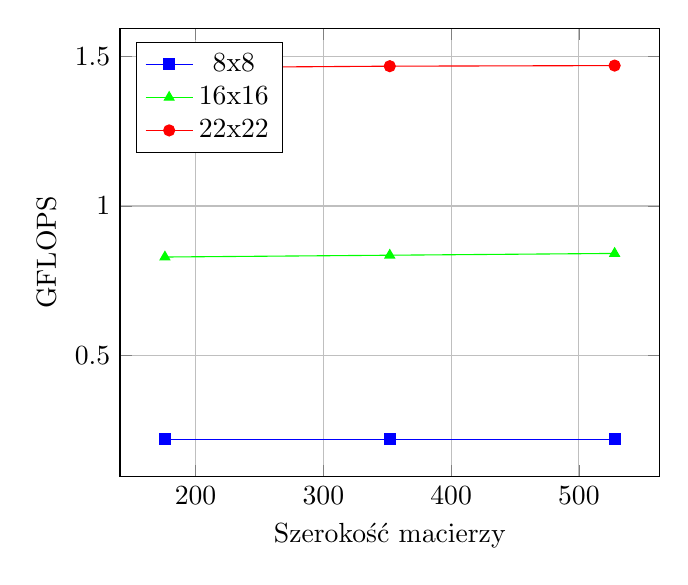
\begin{tikzpicture}
    \begin{axis}[
      xlabel=Szerokość macierzy,ylabel={GFLOPS},legend pos= north west,grid=both]

    \addplot[color=blue,mark=square*] coordinates {%
      (176, 0.219)
      (352, 0.219)
      (528, 0.219)
    };
    \addlegendentry{8x8}

    \addplot[color=green,mark=triangle*] coordinates {%
      (176, 0.829)
      (352, 0.835)
      (528, 0.841)
    };
    \addlegendentry{16x16}

    \addplot[color=red,mark=*] coordinates {%
      (176, 1.463)
      (352, 1.468)
      (528, 1.470)
    };
    \addlegendentry{22x22}

    \end{axis}%
  \end{tikzpicture}%
\caption{Zależność pomiędzy ilością operacji zmiennoprzecinkowychna sekundę a rozmiarem macierzy -- wersja 1.}
\end{figure}

\newpage
\item \textbf{Ilość instrukcji wykonanych na sekundę} \newline

\begin{table}[H]
\centering
\begin{tabular}{|c|c|c|c|}
\hline
\multirow{2}{*}{Rozmiar macierzy} & \multicolumn{3}{c|}{Rozmiar bloku} \\ \cline{2-4}
& 8x8 & 16x16 & 22x22 \\ \hline
176x176 & 0.03798 & 0.14404 & 0.26910 \\ \hline
352x352 & 0.03782 & 0.14434 & 0.26832 \\ \hline
528x528 & 0.03774 & 0.14509 & 0.26820 \\ \hline
\end{tabular}
\caption{Ilość instrukcji wykonana na sekundę (GIPS) -- wersja 1.}
\end{table}

\begin{figure}[H]
\centering
  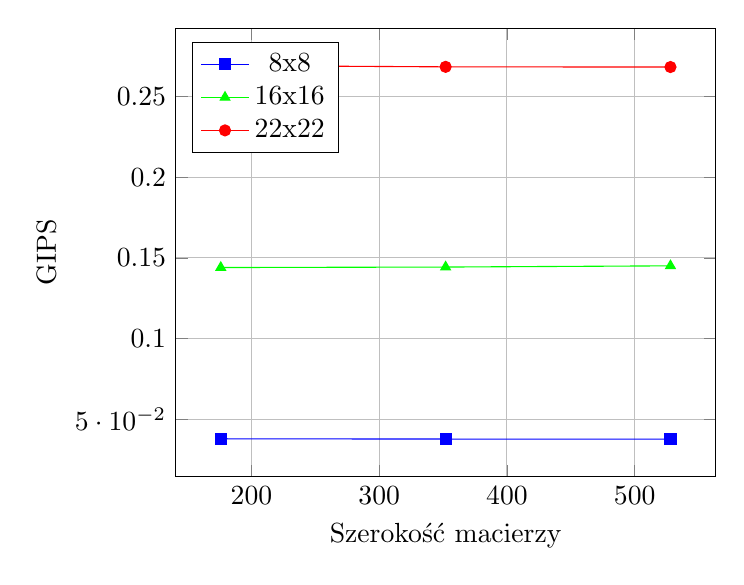
\begin{tikzpicture}
    \begin{axis}[
      xlabel=Szerokość macierzy,ylabel={GIPS},legend pos= north west,grid=both]

    \addplot[color=blue,mark=square*] coordinates {%
      (176, 0.03798)
      (352, 0.03782)
      (528, 0.03774)
    };
    \addlegendentry{8x8}

    \addplot[color=green,mark=triangle*] coordinates {%
      (176, 0.14404)
      (352, 0.14434)
      (528, 0.14509)
    };
    \addlegendentry{16x16}

    \addplot[color=red,mark=*] coordinates {%
      (176, 0.26910)
      (352, 0.26832)
      (528, 0.26820)
    };
    \addlegendentry{22x22}

    \end{axis}%
  \end{tikzpicture}%
\caption{Zależność pomiędzy ilością instrukcji wykonanych na sekundę a rozmiarem macierzy -- wersja 1.}
\end{figure}

\newpage
\item \textbf{CGMA} \newline

\begin{table}[H]
\centering
\begin{tabular}{|c|c|c|c|}
\hline
\multirow{2}{*}{Rozmiar macierzy} & \multicolumn{3}{c|}{Rozmiar bloku} \\ \cline{2-4}
& 8x8 & 16x16 & 22x22 \\ \hline
176x176 & 5.333 & 8.000 & 5.413 \\ \hline
352x352 & 5.333 & 8.000 & 5.414 \\ \hline
528x528 & 5.333 & 8.000 & 5.415 \\ \hline
\end{tabular}
\caption{Stosunek ilości operacji zmiennoprzecinkowych do ilości operacji odczytu/zapisu z pamięci globalnej -- wersja 1.}
\end{table}

\begin{figure}[H]
\centering
  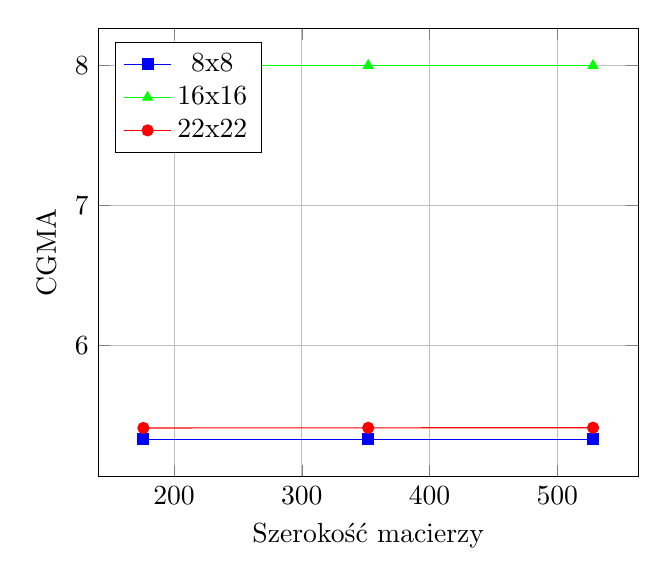
\begin{tikzpicture}
    \begin{axis}[
      xlabel=Szerokość macierzy,ylabel={CGMA},legend pos= north west,grid=both]

    \addplot[color=blue,mark=square*] coordinates {%
      (176, 5.333)
      (352, 5.333)
      (528, 5.333)
    };
    \addlegendentry{8x8}

    \addplot[color=green,mark=triangle*] coordinates {%
      (176, 8.000)
      (352, 8.000)
      (528, 8.000)
    };
    \addlegendentry{16x16}

    \addplot[color=red,mark=*] coordinates {%
      (176, 5.413)
      (352, 5.414)
      (528, 5.415)
    };
    \addlegendentry{22x22}

    \end{axis}%
  \end{tikzpicture}%
\caption{Zależność CGMA od rozmiaru macierzy -- wersja 1.}
\end{figure}

\end{enumerate}
